\chapter{\textcolor{blue}{THE UNCERTAINTY PRINCIPLE}}
  \hspace*{1cm} The uncertainty principle states that the position and velocity cannot both be measured,exactly, at the same time (actually pairs of position, energy and time).\\
\hspace*{1cm}Uncertainty principle derives from the measurement problem, the intimate connection between the wave and particle nature of quantum objects.\\
 \hspace*{1cm}The uncertainty principle is alternatively expressed in terms of a particle's momentum and position. The momentum of a particle is equal to the product of its mass times its velocity($p=mv$). Thus, the product of the uncertainties in the momentum and the position of a particle equals $\hbar/2$ or more. The principle applies to other related (conjugate) pairs of observables, such as energy and time: the product of the uncertainty in an energy measurement and the uncertainty in the time interval during which the measurement is made also equals $\hbar/2$ or more. The same relation holds, for an unstable atom or nucleus, between the uncertainty in the quantity of energy radiated and the uncertainty in the lifetime of the unstable system as it makes a transition to a more stable state.
 \begin{center}
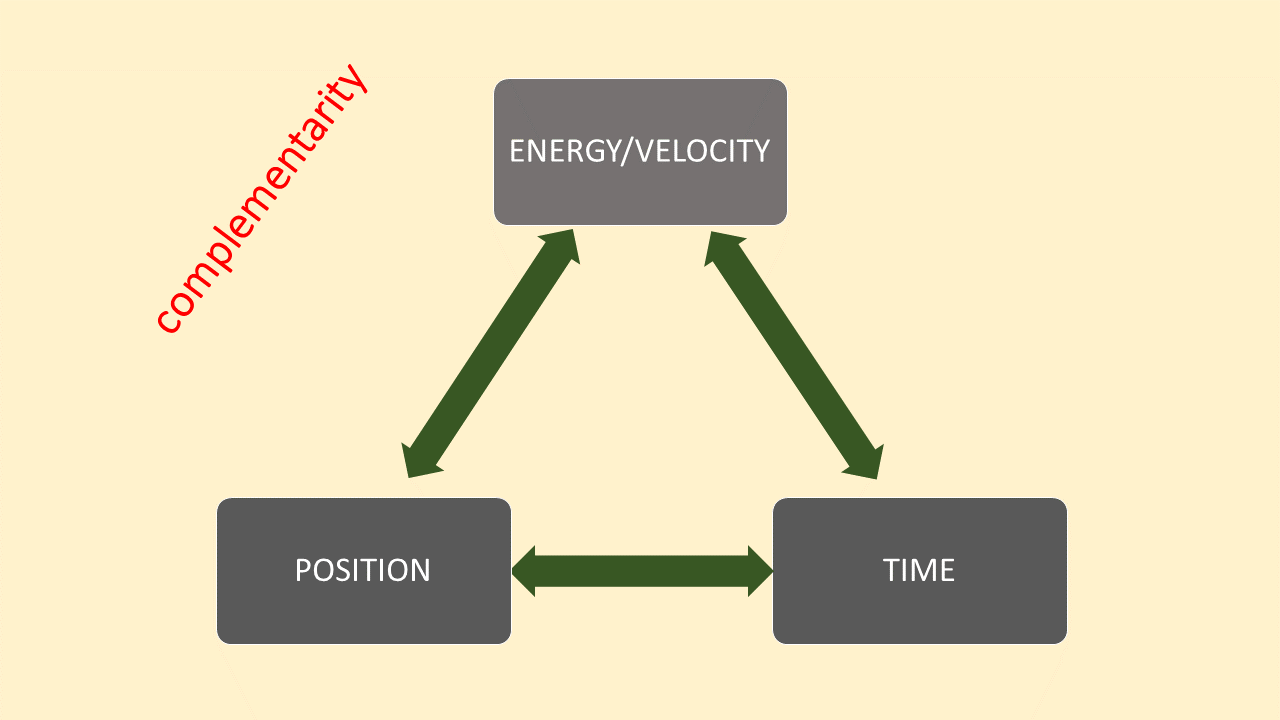
\includegraphics[height=.2\textheight,width=.8\textwidth]{complementarity}
\end{center}
\textbf{Exact knowledge of complementarity pairs (position, energy, time) is impossible.}\\
Mathematically, we describe the uncertainty principle as the following, where ${\sigma}_{x}$ is standard deviation in position 'x' and ${\sigma}_{p}$ is standard deviation in momentum 'p':
$${\sigma}_{x}{\sigma}_{p}\geq \frac{\hbar}{2}$$
In this, I will prove a more general version of the uncertainty principle,and explore some of its implications.
\newpage
\section{Proof of generalized uncertainty principle:-}
\hspace*{10cm} Standard deviation formula for any observable A and B,we have deviation formula for A, $${\sigma}_{A}^{2}=\Braket{(\hat{A}-\Braket{A})\psi|(\hat{A}-\Braket{A})\psi}=\Braket{f|f}$$
where, $f=(\hat{A}-\Braket{A})\psi$ 
and same for B,$${\sigma}_{B}^{2}=\Braket{(\hat{B}-\Braket{B})\psi|(\hat{B}-\Braket{B})\psi}=\Braket{g|g}$$
where, $g=(\hat{B}-\Braket{B})\psi$ 
 $${\sigma}_{A}^{2}{\sigma}_{B}^{2}=\Braket{f|f}\Braket{g|g}$$
 By Schwarz inequality, $${\sigma}_{A}^{2}{\sigma}_{B}^{2}=|\Braket{f|g}|^2$$
 Now $z=x+iy,z^{*}=x-iy$ then $|z|^2=x^2+y^2$ and $Im(z)=\Big[\frac{1}{2i}(z-z^{*})\Big]$\\
 means,$$|z|^2=[Re(z)]^2+[Im(z)]^2\geq [Im(z)]^2=\Big[\frac{1}{2i}(z-z^{*})\Big]^2$$
 Let $z=\Braket{f|g}$,$${\sigma}_{A}^{2}{\sigma}_{B}^{2}\geq \Big[\frac{1}{2i}(\Braket{f|g}-\Braket{g|f})\Big]^2$$
 $$\Braket{f|g}=\Braket{\psi(\hat{A}\hat{B}-\hat{A}\Braket{B}-\hat{B}\Braket{A}+\Braket{A}\Braket{B})\psi}$$
  $$\Braket{f|g}=\Braket{\psi|\hat{A}\hat{B}\psi}-\Braket{B}\Braket{\psi|\hat{A}\psi}-\Braket{A}\Braket{\psi|\hat{B}\psi}+\Braket{A}\Braket{B}\Braket{\psi|\psi}$$
   $$\Braket{f|g}=\Braket{\hat{A}\hat{B}}-\Braket{B}\Braket{\hat{A}}-\Braket{A}\Braket{\hat{B}}+\Braket{A}\Braket{B}$$
      $$\Braket{f|g}=\Braket{\hat{A}\hat{B}}+\Braket{A}\Braket{B}$$
      Similarly,$$\Braket{g|f}=\Braket{\hat{B}\hat{A}}+\Braket{A}\Braket{B}$$
      So,$$\Braket{f|g}-\Braket{g|f}=\Braket{\hat{A}\hat{B}}-\Braket{\hat{B}\hat{A}}$$
      Setting,$[\hat{A},\hat{B}]=\Braket{\hat{A}\hat{B}}-\Braket{\hat{B}\hat{A}}$ is commutator of the two operators\\
     $${\sigma}_{A}^{2}{\sigma}_{B}^{2}\geq \Big(\frac{1}{2i}\Braket{[\hat{A},\hat{B}]}\Big)^2$$
     This is the generalized uncertainty principle.\\
     Now if we choose $A=\hat{x}=x$ and $B=\hat{P}=\frac{\hbar}{i}\frac{d}{dx}$
     $$[\hat{x},\hat{p}]=i\hbar$$
     So,$${\sigma}_{x}^{2}{\sigma}_{p}^{2}\geq \Big(\frac{1}{2i}[\hat{x},\hat{p}]\Big)^2$$
     $${\sigma}_{x}^{2}{\sigma}_{p}^{2}\geq \Big(\frac{1}{2i}{i\hbar}\Big)^2$$
      $${\sigma}_{x}^{2}{\sigma}_{p}^{2}\geq \Big(\frac{\hbar}{2}\Big)^2$$
      Finally,$${\sigma}_{x}{\sigma}_{p}\geq \frac{\hbar}{2}$$
      That's 'THE HEISENBERG UNCERTAINTY PRINCIPLE'.\\
  \textcolor{blue}{ \textbf{PROBLEM 7(3.14):-}Prove the famous "Khatana uncertainty principle," relating the uncertainty in position '$\hat{x}$' to the uncertainty in energy '$\hat{H}$' $$\sigma_{x}\sigma_{H}=\frac{\hbar}{2m}|\Braket{p}|.$$\\
  For stationary state this doesn't tell you much-why not?}\\
  \textbf{Solution:-}\\
  \hspace*{2cm} We know that general  uncertainty principle is $$\sigma_{A}^{2}\sigma_{B}^{2}\geq\Big(\frac{1}{2i}\Braket{\big[\hat{A},\hat{B}\big]}\Big)^2$$
  Here, $\hat{A}=\hat{x}=x$ and $\hat{B}=\hat{H}=-\frac{{\hbar}^2}{2m}\frac{{\partial}^2}{\partial x^2}+V$\\
  Now,\\
  $$\big[\hat{x},\hat{H}\big]g(x)=x\Big(-\frac{{\hbar}^2}{2m}\Big)\frac{{\partial}^2{g}}{\partial {x^2}}-\Big(-\frac{{\hbar}^2}{2m}\Big)\frac{{\partial}^2{gx}}{\partial x^2}$$
  $$\big[\hat{x},\hat{H}\big]g(x)=x\Big(-\frac{{\hbar}^2}{2m}\Big)\frac{{\partial}^2{g}}{\partial {x^2}}+\Big(\frac{{\hbar}^2}{2m}\Big)\frac{{\partial}}{\partial x}\Big(g+{x}\frac{{\partial}g}{\partial x}\Big)$$
   $$\big[\hat{x},\hat{H}\big]g(x)=x\Big(-\frac{{\hbar}^2}{2m}\Big)\frac{{\partial}^2{g}}{\partial {x^2}}+\Big(\frac{{\hbar}^2}{2m}\Big)\Big(\frac{{\partial}g}{\partial x}+\frac{{\partial}g}{\partial x}+{x}\frac{{\partial}^2g}{\partial x^2}\Big)$$
  $$\big[\hat{x},\hat{H}\big]g(x)=\frac{{\hbar}^2}{m}\frac{{\partial}g(x)}{\partial x}$$
  So,\\
  $$\big[\hat{x},\hat{H}\big]=\frac{{\hbar}^2}{m}\frac{{\partial}}{\partial x}$$
  We can write,\\
  $$\big[\hat{x},\hat{H}\big]=\frac{{\hbar}^2}{m}\frac{{\partial}}{\partial x}=\frac{i\hbar}{m}\Big(-i\hbar\frac{{\partial}}{\partial x}\Big)=\frac{i\hbar}{m}{p}$$
  Put the value of $\big[\hat{x},\hat{H}\big]$'\\
  $$\sigma_{H}^{2}\geq\Big(\frac{1}{2i}|\Braket{\frac{i\hbar}{m}{p}}|\Big)$$  
    $$\Rightarrow \sigma_{x}\sigma_{H}\geq\Big(\frac{1}{2i}\frac{i\hbar}{m}\Braket{{p}}\Big)^2$$
    $$\sigma_{x}\sigma_{H}\geq\frac{\hbar}{2m}|\Braket{{p}}|$$
    In stationary state $\sigma_{H}^{2}=0$ because every measurement of the total energy is certain to return the values E.\\
    Also $\Braket{x}=cost.$ , so $\Braket{p}=m\frac{d\Braket{x}}{dt}=0$\\
    $$\therefore  \sigma_{x}\sigma_{H}=0=\frac{\hbar}{2m}|\Braket{{p}}|$$
    \newpage
    \textcolor{blue}{ \textbf{PROBLEM 8(3.17):-} Apply   $\frac{d}{dt}\braket{\Hat{Q}}=\frac{i}{\hbar}\Braket{\big[\hat{H},\hat{Q}]}+\Braket{\frac{\partial{\hat{Q}}}{\partial{t}}}$ to the following spacial case:\\
 (a)$Q=1$;(b)$Q=H$;(c)$Q=x$;(d)$Q=p$.}\\
 \textbf{Solution:-}\\  
 \hspace*{2cm} Given, $$\frac{d}{dt}\braket{\Hat{Q}}=\frac{i}{\hbar}\Braket{\big[\hat{H},\hat{Q}]}+\Braket{\frac{\partial{\hat{Q}}}{\partial{t}}}$$
 And we know that  $$\big[\hat{H},{\hat{p}}\big]={i}{\hbar}\frac{d(V)}{dx}$$
 $$\big[{\hat{H}},x\big]=\frac{i\hbar}{m}{p}$$
  $$\Big[\hat{H},1 \Big]=\hat{H}{1}-{1}\hat{H}=0$$
  and $$\Big[\hat{H},\hat{H} \Big]=\hat{H}\hat{H}-\hat{H}\hat{H}=0$$\\
  Here given all values are explicit time independed, so $$\Braket{\frac{\partial{\hat{Q}}}{\partial{t}}}=0$$ 
  Hence finally,\\
  $$\frac{d}{dt}\braket{1}=0$$
  $$\frac{d}{dt}\braket{\hat{H}}=0$$
   $$\frac{d}{dt}\braket{x}=\frac{\Braket{\hat{p}}}{m}$$
    $$\frac{d}{dt}\braket{\hat{p}}=-\Braket{\frac{\partial {V}}{\partial{x}}}$$
   The last equestion is  \textbf{`EHRENFEST'S THEOREM'.}
  \newpage
   \textcolor{blue}{ \textbf{PROBLEM 9(3.31):-}  \textbf{(VIRIAL THEOREM)} \\
   $$\frac{d}{dx}\Braket{xp}=2\Braket{T}-\Big{\langle}x\frac{dV}{dx}\Big{\rangle}$$
   where T is the kinetic energy(H=T+V).In the stationary state the left side is zero so\\
   $$2\Braket{T}=\Big{\langle}x\frac{dV}{dx}\Big{\rangle}$$
   This is called the '\textbf{VIRIAL THEOREM}'.Use it and prove that $\Braket{T}=\Braket{V}$ for stationary state harmonic oscillator.}\\
   \textbf{Solution:-}\\
   \hspace*{2cm} First we find $\frac{d{\Braket{x\hat{p}}}}{dt}$\\
    $$\frac{d{\Braket{x\hat{p}}}}{dt}=\frac{d}{dt}{\Braket{\psi|x\hat{p}\psi}}$$
   $$\frac{d{\Braket{x\hat{p}}}}{dt}={\Braket{\frac{d\psi}{dt}|x\hat{p}\psi}}+{\Braket{\psi|\frac{dx\hat{p}}{dt}{\psi}}}+{\Braket{\psi|{x\hat{p}}\frac{d\psi}{dt}}}$$
  Here $\hat{x}=x$ and $\hat{p}=\frac{h}{i}\frac{d}{dx}$,
   $$x\hat{p}=x\Big(\frac{h}{i}\frac{d}{dx}\Big)$$
   $$\frac{dx\hat{p}}{dt}=\frac{d}{dt}\Big(\frac{xh}{i}\frac{d}{dx}\Big)=0$$
    $$\frac{d{\Braket{x\hat{p}}}}{dt}={\Braket{\frac{d\psi}{dt}|x\hat{p}\psi}}+{\Braket{\psi|{x\hat{p}}\frac{d\psi}{dt}}}$$
    We know that, $\hat{H}=i\hbar\frac{\partial}{\partial{t}}$
    $$\hat{H}{\psi}=i\hbar\frac{\partial{\psi}}{\partial{t}}\Rightarrow \frac{\partial{\psi}}{\partial{t}}=\frac{1}{i\hbar}\hat{H}{\psi}$$
   $$\frac{d{\Braket{x\hat{p}}}}{dt}={\Braket{\frac{1}{i\hbar}\hat{H}{\psi}|x\hat{p}\psi}}+{\Braket{\psi|{x\hat{p}}\frac{1}{i\hbar}\hat{H}{\psi}}}$$
   $$\frac{d{\Braket{x\hat{p}}}}{dt}=-\frac{1}{i\hbar}{\Braket{\hat{H}{\psi}|x\hat{p}\psi}}+\frac{1}{i\hbar}{\Braket{\psi|{x\hat{p}}\hat{H}{\psi}}}$$
   We know that $\hat{H}$ is hermition ,so ${\Braket{\hat{H}{\psi}|x\hat{p}\psi}}={\Braket{{\psi}|\hat{H}x\hat{p}\psi}}$\\
   $$\frac{d{\Braket{x\hat{p}}}}{dt}=-\frac{1}{i\hbar}{\Braket{{\psi}|\hat{H}x\hat{p}\psi}}+\frac{1}{i\hbar}{\Braket{\psi|{x\hat{p}}\hat{H}{\psi}}}$$
   $$\frac{d{\Braket{x\hat{p}}}}{dt}=\frac{i}{\hbar}{\Braket{{\psi}|\hat{H}x\hat{p}\psi}}-\frac{i}{\hbar}{\Braket{\psi|{x\hat{p}}\hat{H}{\psi}}}$$
   $$\frac{d{\Braket{x\hat{p}}}}{dt}=\frac{i}{\hbar}\Big[{\Braket{{\psi}|\hat{H}x\hat{p}\psi}}-\Braket{\psi|{x\hat{p}}\hat{H}{\psi}}\Big]$$
    $$\frac{d{\Braket{x\hat{p}}}}{dt}=\frac{i}{\hbar}\Braket{\big[{\hat{H},x\hat{p}}\big]}$$
    Now$$\big[{\hat{H},x\hat{p}}\big]={\hat{H}x\hat{p}}-x\hat{H}\hat{p}+x\hat{H}\hat{p}-{x\hat{p}\hat{H}}$$
    $$\big[{\hat{H},x\hat{p}}\big]=\big({\hat{H}x}-x\hat{H}\big)\hat{p}+x\big(\hat{H}\hat{p}-{\hat{p}\hat{H}}\big)$$
    $$\big[{\hat{H},x\hat{p}}\big]=\big[{\hat{H}},x\big]\hat{p}+x\big[\hat{H},{\hat{p}}\big]$$
    We know that $$\big[{\hat{H}},x\big]=\frac{i\hbar}{m}{p}$$
    and
    $$\big[\hat{H},{\hat{p}}\big]=\Big[\frac{p^2}{2m}+V,{\hat{p}}\Big]$$
     $$\big[\hat{H},{\hat{p}}\big]=\Big[\frac{p^2}{2m},{\hat{p}}\Big]+\big[V,{\hat{p}}\big]$$
     $$\big[\hat{H},{\hat{p}}\big]=\frac{p^2}{2m}{\hat{p}}-{\hat{p}}\frac{p^2}{2m}+\big[V,{\hat{p}}\big]$$
       $$\big[\hat{H},{\hat{p}}\big]=\big[V,{\hat{p}}\big]$$
    Now we find $\big[V,{\hat{p}}\big]$,\\
    $$\big[V,{\hat{p}}\big]f=V\frac{\hbar}{i}\frac{df}{dx}-\frac{\hbar}{i}\frac{d(Vf)}{dx}$$
    $$\big[V,{\hat{p}}\big]f=V\frac{\hbar}{i}\frac{df}{dx}-V\frac{\hbar}{i}\frac{df}{dx}-{f}\frac{\hbar}{i}\frac{d(V)}{dx}$$
       $$\big[V,{\hat{p}}\big]f=-{f}\frac{\hbar}{i}\frac{d(V)}{dx}$$
       $$\big[V,{\hat{p}}\big]f={i}{\hbar}\frac{d(V)}{dx}{f}$$
        $$\big[V,{\hat{p}}\big]={i}{\hbar}\frac{d(V)}{dx}$$
       $$\big[\hat{H},{\hat{p}}\big]={i}{\hbar}\frac{d(V)}{dx}$$
       $$\frac{d{\Braket{x\hat{p}}}}{dt}=\frac{i}{\hbar}\Bigg[-\frac{i\hbar}{m}\Braket{p^2}+i{\hbar}\Braket{x\frac{dV}{dx}}\Bigg]$$
        $$\frac{d{\Braket{x\hat{p}}}}{dt}=\Bigg[\frac{1}{m}\Braket{p^2}-\Braket{x\frac{dV}{dx}}\Bigg]$$
       $$\frac{d{\Braket{x\hat{p}}}}{dt}=2\Braket{\frac{p^2}{2m}}-\Braket{x\frac{dV}{dx}}$$
       We know that $T=\frac{1}{2}m{v^2}$ and $p=mv$.\\ So, $T=\frac{p^2}{2m}.$\\
         $$\frac{d{\Braket{x\hat{p}}}}{dt}=2\Braket{T}-\Braket{x\frac{dV}{dx}}$$
       Here $\Braket{x\hat{p}}$ is not depend on 't'\\ So, $\frac{d{\Braket{x\hat{p}}}}{dt}=0$
       \[\boxed{$$ 2\Braket{T}=\Braket{x\frac{dV}{dx}}$$}\]
       Here V is potential energy,$V(X)=\frac{1}{2}{kx^2}$ and here k is spring force constant.\\
       And we know $\omega$ is the (anguler) frequency of oscillation, $\omega=\sqrt{\frac{k}{k}}\Rightarrow k=m{\omega}^2$\\
       then,$$V(X)=\frac{1}{2}m{\omega}^2{x^2} \Rightarrow \frac{dV}{dx} =m{\omega}^2{x}$$
       $$\frac{d{\Braket{x\hat{p}}}}{dt}=2\Braket{T}-\Braket{m{\omega}^2{x}^2}$$
       $$\frac{d{\Braket{x\hat{p}}}}{dt}=2\Braket{T}-\Braket{2V}=2\Braket{T}-2\Braket{V}$$
       Therefore, $$\Braket{T}=\Braket{V}$$
 \newpage
 \textcolor{blue}{ \textbf{PROBLEM 10(3.34):-}  \textbf{(Coherent states of the harmonic oscillator).} \\Among the stationary states of the harmonic oscillator ($\ket{n}={\psi}_{n}(x)$),
 $${\psi}_{n}=\frac{1}{\sqrt{n!}}(a_{+})^n{{\psi}_{0}}$$
 only $n=0$ hits the uncertainty limit $({\sigma}_{x} {\sigma}_{p}=\hbar/2)$;in general;${\sigma}_{x} {\sigma}_{p}=(2n+1)\hbar/2$, as you found earlier examples .But certain linear combination (known as coherent states) also minimize the uncertainty product.they are(as it turns out) eigenvafunctions of the lowering operator:$$a_{-}\ket{\alpha}=\alpha\ket{\alpha}$$ (the eigenvalue $\alpha$ can be any complex number).\\
 \textbf{(a)} Calculate $\Braket{x}$, $\Braket{x^2}$, $\Braket{p}$ and $\Braket{p^2}$ in the state $\ket{\alpha}$ .\\Hint: Remember that ${\alpha}_{-}$ is the hermitian conjugate  of ${\alpha}_{-}$,and do not assume $\alpha$ is real.\\
 \textbf{(b)} Find ${\Sigma}_{x}$ and ${\Sigma}_{p}$ ;show that ${\Sigma}_{x}{\Sigma}_{p}=\hbar/2.$\\
 \textbf{(c)} like any other wave function, a coherent state can be expanded in terms of energy eigenstates:
 $$\ket{\alpha}=\sum_{n=0}^{\infty} c_{n}\ket{n}.$$ 
 Show that the expansion coefficients are 
 $$c_{n}=\frac{{\alpha}^n}{\sqrt{n!}}c_{0}.$$
 \textbf{(d)} Determine $c_{0}$ by normalizing $\ket{\alpha}$\\
 \textbf{(e)} Now put in the time dependence:
 $$\ket{n}{\rightarrow} e^{iE_{n}t/h}\ket{n},$$
 and show that that $\ket{\alpha{(t)}}$ remains an eigenstates of $a_{-}$, but the eigenvalue evolves in time:
 $$\alpha{(t)}=e^{i{\omega} {t}}{\alpha}.$$
 So a coherent state stays coherent, and continues to minimize the uncertainty product.}\\
  \textbf{Solution:-}\\
 \hspace*{3cm}\textbf{(a)} $$\Braket{\hat{x}}=\Braket{\alpha|\hat{x}\alpha}$$
 We know that$$\hat{x}=\sqrt{\frac{\hbar}{2m\omega}}(a_{+}+a_{-})$$
 then $$\Braket{\hat{x}}=\Braket{\alpha|\sqrt{\frac{\hbar}{2m\omega}}(a_{+}+a_{-})\alpha}$$
 $$\Braket{\hat{x}}=\sqrt{\frac{\hbar}{2m\omega}}\Braket{\alpha|(a_{+}+a_{-})\alpha}$$
  $$\Braket{\hat{x}}=\sqrt{\frac{\hbar}{2m\omega}}\Big(\Braket{\alpha|a_{+}\alpha}+\Braket{\alpha|a_{-}\alpha}\big)$$
  $$\Braket{\hat{x}}=\sqrt{\frac{\hbar}{2m\omega}}\Big(\alpha\Braket{\alpha|\alpha}+{\alpha}^{*}\Braket{\alpha|\alpha}\big)$$
 $$\Braket{\hat{x}}=\sqrt{\frac{\hbar}{2m\omega}}\Big(\alpha+{\alpha}^{*}\big)$$
 $$\Braket{(\hat{x})^2}=\Braket{\alpha|(\hat{x})^2\alpha}$$
 We know that$$\hat{(x)^2}={\frac{\hbar}{2m\omega}}(a_{+}^{2}+a_{-}^{2}+a_{+}a_{-}+a_{-}a_{+})$$
 and$$ [a_{-},a_{+}]=a_{-}a_{+}-a_{+}a_{-}$$
 $$a_{-}a_{+}=[a_{-},a_{+}]+a_{+}a_{-}$$
 $$a_{-}a_{+}=1+a_{+}a_{-}$$
 Now,$$[a_{-},a_{+}]=1(?)$$
 $$ [a_{-},a_{+}]\ket{n}=(a_{-}a_{+}-a_{+}a_{-})\ket{n}$$
 We know that, $a_{-}\ket{n}=\sqrt{n}\ket{n-1}$ and  $a_{+}\ket{n}=\sqrt{n+1}\ket{n+1}$\\
  $$ [a_{-},a_{+}]\ket{n}=a_{-}a_{+}\ket{n}-a_{+}a_{-}\ket{n}$$
 $$ [a_{-},a_{+}]\ket{n}=a_{-}(\sqrt{n+1}\ket{n+1})-a_{+}(\sqrt{n}\ket{n-1})$$
  $$ [a_{-},a_{+}]\ket{n}=\sqrt{n+1}(a_{-}\ket{n+1})-\sqrt{n}(a_{+}\ket{n-1})$$
 $$ [a_{-},a_{+}]\ket{n}=\sqrt{n+1}\sqrt{n+1}\ket{n}-\sqrt{n}\sqrt{n}\ket{n}$$
  $$ [a_{-},a_{+}]\ket{n}={(n+1)}\ket{n}-{(n)}\ket{n}$$
  $$ [a_{-},a_{+}]\ket{n}={((n+1)-(n))}\ket{n}$$
  $$ [a_{-},a_{+}]\ket{n}=\ket{n}$$
  $$ [a_{-},a_{+}]=1.$$
  $$\hat{(x)^2}={\frac{\hbar}{2m\omega}}(a_{+}^{2}+a_{-}^{2}+2a_{+}a_{-}+1)$$
 $$\Braket{(\hat{x})^2}={\frac{\hbar}{2m\omega}}\Braket{\alpha|(a_{+}^{2}+a_{-}^{2}+2a_{+}a_{-}+1)\alpha}$$
 $$\Braket{(\hat{x})^2}={\frac{\hbar}{2m\omega}}\Big[{{\alpha}^*}^2+2{\alpha}^*{\alpha}+{\alpha}^2+1\Big]$$
 $$\Braket{(\hat{x})^2}={\frac{\hbar}{2m\omega}}\Big[({{\alpha}+{\alpha}^*})^2+1\Big]$$
 
 $$\Braket{\hat{p}}=\Braket{\alpha|\hat{x}\alpha}$$
 We know that$$\hat{x}=i\sqrt{\frac{m\omega\hbar}{2}}(a_{+}-a_{-})$$
 then $$\Braket{\hat{x}}=\Braket{\alpha|i\sqrt{\frac{m\omega\hbar}{2}}(a_{+}-a_{-})\alpha}$$
 $$\Braket{\hat{x}}=i\sqrt{\frac{m\omega\hbar}{2}}\Braket{\alpha|(a_{+}-a_{-})\alpha}$$
  $$\Braket{\hat{x}}=i\sqrt{\frac{m\omega\hbar}{2}}\Big(\Braket{\alpha|a_{+}\alpha}-\Braket{\alpha|a_{-}\alpha}\big)$$
  $$\Braket{\hat{x}}=i\sqrt{\frac{m\omega\hbar}{2}}\Big(\Braket{{\alpha}^{*}\alpha|\alpha}-\alpha\Braket{\alpha|\alpha}\big)$$
  $$\Braket{\hat{p}}=-i\sqrt{m\omega\frac{\hbar}{2}}\Big(\alpha-{\alpha}^{*}\big)$$

$$\Braket{(\hat{p})^2}=\Braket{\alpha|(\hat{p})^2\alpha}$$
 We know that$$\hat{(p)^2}={-\frac{m\omega\hbar}{2}}(a_{+}^{2}+a_{-}^{2}-a_{+}a_{-}-a_{-}a_{+})$$
 and$$a_{-}a_{+}=1+a_{+}a_{-}$$

$$\hat{(p)^2}={-\frac{m\omega\hbar}{2}}(a_{+}^{2}+a_{-}^{2}-2a_{+}a_{-}-1)$$
 $$\Braket{(\hat{p})^2}={-\frac{m\omega\hbar}{2}}\Braket{\alpha|(a_{+}^{2}+a_{-}^{2}-2a_{+}a_{-}-1)\alpha}$$
 $$\Braket{(\hat{p})^2}={-\frac{m\omega\hbar}{2}}\Big[{{\alpha}^*}^2-2{\alpha}^*{\alpha}+{\alpha}^2-1\Big]$$
 $$\Braket{(\hat{p})^2}={-\frac{m\omega\hbar}{2}}\Big[({{\alpha}-{\alpha}^*})^2-1\Big]$$
 $$\Braket{(\hat{p})^2}={\frac{m\omega\hbar}{2}}\Big[1-({{\alpha}-{\alpha}^*})^2\Big]$$
\hspace*{3cm}\textbf{(b)} $${\sigma}_{x}^{2}=\Braket{x^2}+{\Braket{x}}^2={\frac{\hbar}{2m\omega}}\Big[1+({{\alpha}+{\alpha}^*})^2-\big(\alpha+{\alpha}^{*}\big)^2\Big]$$ 
  $${\sigma}_{x}^{2}=\Braket{x^2}+{\Braket{x}}^2={\frac{\hbar}{2m\omega}}$$
 
 $${\sigma}_{p}^{2}=\Braket{p^2}+{\Braket{p}}^2={\frac{m\omega\hbar}{2}}\Big[1-({{\alpha}-{\alpha}^*})^2+\big(\alpha-{\alpha}^{*}\big)^2\Big]$$ 
  $${\sigma}_{p}^{2}=\Braket{x^2}+{\Braket{x}}^2={\frac{m\omega\hbar}{2}}$$
  Thus$${\sigma}_{x}{\sigma}_{p}=\sqrt{\frac{\hbar}{2m\omega}}\sqrt{\frac{m\omega\hbar}{2}}=\frac{\hbar}{2}$$
  
  \textbf{(c)} \\
  \hspace*{1cm}We know that
  $$\ket{\alpha}={\sum}_{0}^{\infty}c_{n}\ket{n}$$
  In harmonic ascillator $$a_{+}\ket{n}=\sqrt{n+1}\ket{n+1}$$
  $$a_{+}^{n}\ket{{\psi}_{0}}=\sqrt{n!}\ket{n}$$
  $$\ket{n}=\frac{a_{+}^{n}}{\sqrt{n!}}\ket{{\psi}_{0}}$$
  then\\ $$\ket{\alpha}={\sum}_{0}^{\infty}c_{n}\frac{a_{+}^{n}}{\sqrt{n1}}\ket{{\psi}_{0}}$$
  Now,$$c_{n}=\Braket{n|\alpha}=\Braket{\frac{a_{+}^{n}}{\sqrt{n!}}{\psi}_{0}|\alpha}=\frac{1}{\sqrt{n!}}\Braket{{a_{+}^{n}}{\psi}_{0}|\alpha}$$
  $$c_{n}=\frac{1}{\sqrt{n!}}\Braket{{\psi}_{0}|{a_{-}^{n}}\alpha}$$
  $$c_{n}=\frac{{\alpha}^n}{\sqrt{n!}}\Braket{{\psi}_{0}|\alpha}=\frac{{\alpha}^n}{\sqrt{n!}}c_{0}$$
    $$\therefore c_{n}=\frac{{\alpha}^n}{\sqrt{n!}}c_{0}$$
  
  \textbf{(d)} \\
  \hspace*{1cm}We know that $\Braket{\alpha|\alpha}=1$,\\
  then$$\Braket{\alpha|\alpha}=\sum_{0}^{\infty}c_{n}{c_{n}}^*\Braket{n|n}=\sum_{0}^{\infty}|{c_{n}}|^2=1$$
  Put $c_{n}=\frac{{\alpha}^n}{\sqrt{n!}}c_{0}$,then
  $$\Rightarrow\sum_{0}^{\infty}\frac{|{\alpha}|^2n}{{n!}}{c_{0}}^2=1$$
    $$\Rightarrow {c_{0}}^2 \sum_{0}^{\infty}\frac{\Big(|{\alpha}|^2\Big)^2}{{n!}}=1$$
   $$\Rightarrow {c_{0}}^2 {e}^{{|\alpha|}^2}=1$$
   $$\therefore  {c_{0}}= e^{{-{|\alpha|}^2}/{2}}$$
  
  \textbf{(e)} \\
  \hspace*{2cm} Given $\ket{n}\rightarrow e^{-iE_{n}t/{\hbar}}\ket{n} $then,
  $$\ket{\alpha(t)}={\sum}_{0}^{\infty}c_{n}e^{-iE_{n}t/{\hbar}}\ket{n}$$
  Put $c_{n}=\frac{{\alpha}^n}{\sqrt{n!}}c_{0}$,
  
  $$\ket{\alpha(t)}={\sum}_{0}^{\infty}\Big(\frac{{\alpha}^n}{\sqrt{n!}}c_{0}\Big)e^{-iE_{n}t/{\hbar}}\ket{n}$$
  Put ${c_{0}}= {e}^{{-{|\alpha|}^2}/{2}}$,
  $$\ket{\alpha(t)}={\sum}_{0}^{\infty}\Big(\frac{{\alpha}^n}{\sqrt{n!}}\Big){e}^{{-{|\alpha|}^2}/{2}}e^{-iE_{n}t/{\hbar}}\ket{n}$$
  $$\ket{\alpha(t)}={\sum}_{0}^{\infty}\Big(\frac{{\alpha}^n}{\sqrt{n!}}\Big)e^{-({{|\alpha|}^2}/{2}+iE_{n}t/{\hbar})}\ket{n}$$
  Now in harmonic oscillator,$E_{n}=\Big(n+\frac{1}{2}\Big)\hbar\omega$\\
  Here $E_{n}$ energy of $n^{th}$ excited states of harmonic oscillator.\\
   $$\ket{\alpha(t)}={\sum}_{0}^{\infty}\Big(\frac{{\alpha}^n}{\sqrt{n!}}\Big){e}^{{-{|\alpha|}^2}/{2}}e^{-i{\Big(n+\frac{1}{2}\Big)\omega}t}\ket{n}$$
  
     $$\ket{\alpha(t)}={\sum}_{0}^{\infty}\Big(\frac{{\alpha}^n}{\sqrt{n!}}\Big){e}^{{-{|\alpha|}^2}/{2}}e^{-i{n\omega}t}e^{-\frac{i}{2}{\omega}t}\ket{n}$$
  
     $$\ket{\alpha(t)}=e^{-\frac{i}{2}{\omega}t}{\sum}_{0}^{\infty}\Big(\frac{({\alpha{e^{-i{\omega}t}}})^n}{\sqrt{n!}}\Big){e}^{{-{|\alpha|}^2}/{2}}\ket{n}$$
  
  Apartfrom the overall phase factor $e^{-\frac{i}{2}{\omega}t}$(which dose not affect  its status as an eigenfunction of $a_{-}$,0r its eigenvalue),$\ket{\alpha(t)}$ is the same as $\ket{\alpha}$, but with eigenvalue $\alpha(t)=e^{-\frac{i}{2}{\omega}t}\alpha$.\\
  
  \textbf{(e)} \\
  \hspace*{2cm} By applying lowering operator on ground states of harmonic oscillator,\\
 $$a_{-}{\psi}_{0}=0$$ or$$a_{-}\ket{{\psi}_{0}}$$\S0, YES it is a coherent state,which eigenvalue $\alpha=0$